\documentclass[notheorems]{beamer}
\usepackage{SlideStyle}
\usepackage{mathtools}
\usepackage{graphicx}
\newcommand{\Binom}{\operatorname{Binom}}
\renewcommand{\d}{\operatorname{d}}

\titlegraphic{\vspace*{-7cm}
    \parbox[c]{3cm}{
\includegraphics[height=.7cm]{bsulogo}}
    \hspace*{1cm}%
    \parbox[c]{2cm}{
\includegraphics[height=0.6cm]{FPMIlogo_new}}
    \hspace*{1cm}%
    \vspace*{3cm}
}

\title[Модели распространения заболеваний]{Отчет по преддипломной практике \\ \Large CТАТИСТИЧЕСКИЙ АНАЛИЗ РАСПРОСТРАНЕНИЯ ЗАБОЛЕВАНИЙ}


\author[В. А. Гут]{Гут Валерия Александровна}

\institute[]{Научный руководитель: С.В. Лобач}


\date[]{}%{\scriptsize \structure{2017-2018}}


\begin{document}

\begin{frame}[plain]
  \titlepage
\end{frame}


%--------------------------------------------------------------------------------------
\begin{frame}{Цели и задачи работы}

1. изучение рекомендованной литературы;

2. изучение предложенных в литературе алгоритмов;

3. компьютерная реализация алгоритмов;

4. сравнение алгоритмов;

5. подготовка отчета и презентации.


\end{frame}

%--------------------------------------------------------------------------


\begin{frame}
	{SEIR-модель}
	\small{В SEIR модели предполагается, что инфекция имеет инкубационный период, в течение которого люди инфицированы, но
	еще не заразны. Эта группа людей обозначается через $E$ (exposed). С учетом нового класса получаем следующую структуру
	популяции:
	$$S + E + I + R = N,$$ где
	\begin{itemize}
		\item $S(t)$ -- это количество не инфицированных людей, $\beta$ -- это скорость передачи заболевания;
		\item $E(t)$ -- это число инфицированных, но еще не заразных людей.  Параметр $\sigma^{-1}$ представляет собой среднюю продолжительность инкубационного периода;
		\item $I(t)$ -- это количество инфицированных людей. Параметр $\gamma$ -- это скорость восстановления;
		\item $R(t)$ -- это группа выздоровевших лиц, а именно людей, которые восстановились.
	\end{itemize}
}
\end{frame}


%--------------------------------------------------------------------------

\begin{frame}
	{SEIR-модель}
	Классическая SEIR-модель описывается задачей Коши
	Модель SEIR описывается задачей Коши
	\begin{equation*}
		\begin{dcases}
			\dfrac {\d S(t)}{\d t} = - \beta \cdot I(t)\cdot S(t),\\
			\dfrac {\d E(t)}{\d t} = \beta \cdot S(t)\cdot I(t) - \sigma\cdot E(t),\\
			\dfrac{\d I(t)}{\d t} =\sigma \cdot E(t) - \gamma\cdot I(t),\\
			\dfrac{\d R(t)}{\d t} = \gamma\cdot I(t),\\
			S(0) = S_0,\ I(0) = I_0,\ E(0) = 0,\ R(0) = 0.
		\end{dcases}
	\end{equation*}
	Эту SEIR-модель мы будем называть \textit{детерминированной}.
\end{frame}

%--------------------------------------------------------------------------

\begin{frame}
	{Моделирования процесса распространения гриппа. Постановка задачи
	}
	Симптомы гриппа появляются на \textbf{1—4-й день} после заражения и включают в себя лихорадку, кашель, головную боль, боль в мышцах и суставах, слабость, боль в горле и насморк. При этом кашель может длиться две и более недели. Наиболее заразен больной на \textbf{3—4-й день} с момента появления симптомов. Реконвалесцентный период составляет \textbf{7—15 дней}. После выздоровления формируется иммунитет к конкретному штамму вируса, но он не защищает от других штаммов. Иммунитет носит временный характер (обычно до \textbf{1-2 лет}).
\end{frame}

%--------------------------------------------------------------------------

\begin{frame}
	{Входные данные}
\small {На основе приведенной информации о распространении можем сформулировать математическую модель следующим образом. Так как симптомы появляются через 1-4 дня, то возьмем средний инкубационный период для модели $T_\text{инкубац} = 2$ дня. Тогда коэффициент перехода из $E$ в $I$ равна
$$\sigma = \dfrac{1}{T_\text{инкубац}} = \dfrac 1 2 = 0.5.$$
Средний инфекционный период выберем $T_\text{инфекц}=5$ дней.
Тогда коэффициент выздоровления равен
$$\gamma = \dfrac{1}{T_\text{инфекц}} = \dfrac 1 5 = 0.2.$$
Коэффициент передачи инфекции $\beta$ мы можем получить из  базового репродуктивного числа через следующее соотношение
$$\beta = R_0\cdot \gamma = 1.5\cdot 0.2 = 0.3.$$

В качестве числа населения возьмем $N=1000$, а число инфицированных зададим равное $I_0 = 20$. Отсюда $S_0 = N - I_0 = 980$. Данный процесс будем рассматривать в течение $T=100$ дней.}
\end{frame}

%--------------------------------------------------------------------------

\begin{frame}
	{Применение детерминированной SEIR модели для моделирования}
	Ввиду входных условий, получаем систему дифференциальных уравнений модели SEIR
	\begin{equation*}
		\begin{dcases}
			\dfrac {\d S(t)}{\d t} = - 0.3 \cdot I(t)\cdot S(t),\\
			\dfrac {\d E(t)}{\d t} = 0.3 \cdot S(t)\cdot I(t) - 0.5\cdot E(t),\\
			\dfrac{\d I(t)}{\d t} =0.5 \cdot E(t) - 0.2\cdot I(t),\\
			\dfrac{\d R(t)}{\d t} = 0.2\cdot I(t),\\
			S(0) = 980,\ I(0) = 20,\ E(0) = 0,\ R(0) = 0.
		\end{dcases}
	\end{equation*} 
	
	Ее решение вычисляется с помощью численных методов.
\end{frame}

%--------------------------------------------------------------------------
\begin{frame}
	{Применение детерминированной SEIR модели для моделирования}
\begin{figure}
	\centering
	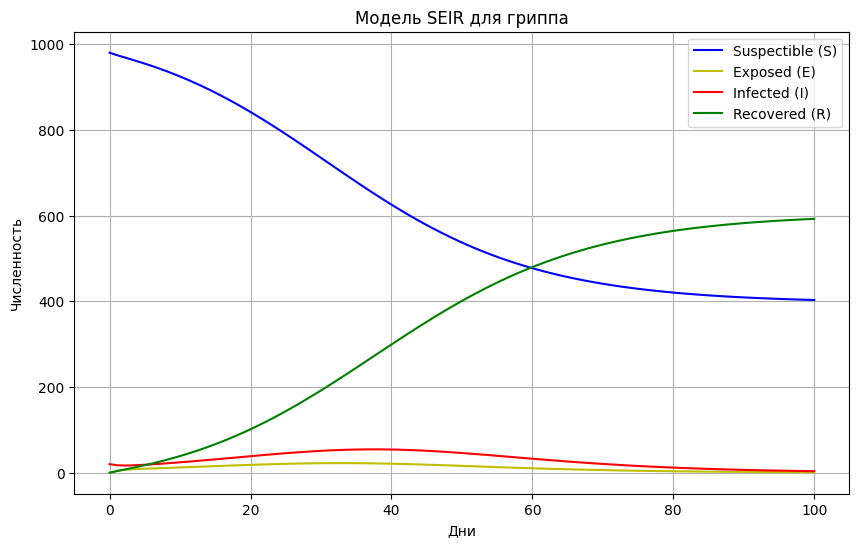
\includegraphics[scale=0.4]{images/graph01}
	\caption{График численного решения задачи Коши для детерминированной SEIR модели}
	\label{fig:graph01}
\end{figure}
\end{frame}

%--------------------------------------------------------------------------

\begin{frame}
	{Вероятностные популяционные модели}
	\small{Построим вероятностную модель с дискретным временем, поскольку для нее легко привести численную реализацию. Вероятностная SEIR-модель для гриппа имеет следующий вид
	\begin{equation}
		\begin{dcases}
			S_{t+1} = S_t - \Delta E_t,\\
			E_{t+1} = E_t +\Delta E_t - \Delta I_t,\\
			I_{t+1} = I_t + \Delta I_t - \Delta R_t,\\
			R_{t+1} = R_t + \Delta R_t,
			S_0 = 980,\ E_0 = 0,\ I_0 = 20,\ \ R_0 = 0
		\end{dcases}
		t = 0,1,2\ldots,
	\end{equation}
	при этом
	$$\Delta E_t \sim \Binom\left(S_t, 
	1 - \exp\left(-\beta\cdot  \frac{I}{N} \cdot \Delta t\right)\right),$$
	$$\Delta I_t \sim \Binom\left(E_t, 1 - \exp\left(-\sigma \cdot \Delta t\right)\right),$$
	$$\Delta R_t \sim \Binom\left(I_t, 1 - \exp\left(-\gamma \cdot \Delta t\right)\right).$$
	
	Таким образом, мы можем описать процесс распространения гриппа с помощью вероятностной SEIR модели. Приведем 100 реализаций этой модели, а в качестве результирующего графика выберем средние значения для каждой группы, а также приведем 95\%-доверительные интервалы для каждой переменной}
\end{frame}

%--------------------------------------------------------------------------

\begin{frame}
	{Вероятностные популяционные модели}
	\begin{figure}
		\centering
		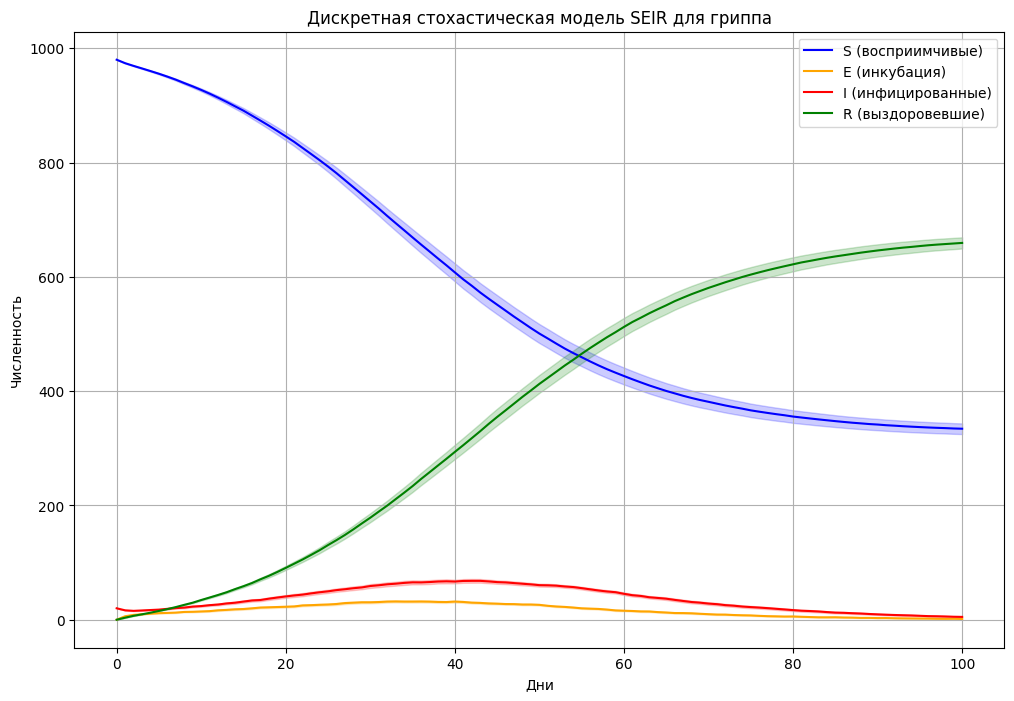
\includegraphics[scale=0.4]{images/graph02}
		\caption{График численной реализация вероятностной SEIR для гриппа с доверительными интервалами}
		\label{fig:graph02}
	\end{figure}
	
\end{frame}

%--------------------------------------------------------------------------

\begin{frame}
	{Постановка задачи для пространственной модели}
	Клеточные автоматы -- это удобный инструмент для моделирования пространственных процессов, таких как распространение инфекции. В такой модели
	
	\begin{itemize}
		\item пространство делится на дискретные ячейки (регион, квартал, город и т.д.);
		\item каждая ячейка имеет состояние (например, $S$, $E$, $I$, $R$);
		\item состояние каждой ячейки обновляется во времени в зависимости от её текущего состояния и состояния соседей.
	\end{itemize}
	
	Клеточные автоматы хорошо подходят для моделирования локальных взаимодействий и пространственного распространения инфекции.
\end{frame}
%--------------------------------------------------------------------------

\begin{frame}{Применение пространственной SEIR модели для моделирования}
	\small{Для пространственной модели построим сетку узлов $30 \times 30$ на которой зададим вероятностную SEIR-модель для дискретного времени с сохранением всех параметров из предыдущего случая. Клетки, в которых будут находиться инфицированные люди, будут выбираться случайно.}
	
	
\end{frame}

%--------------------------------------------------------------------------

\begin{frame}
	
	{Применение пространственной SEIR модели для моделирования}
	\begin{figure}
		\centering
		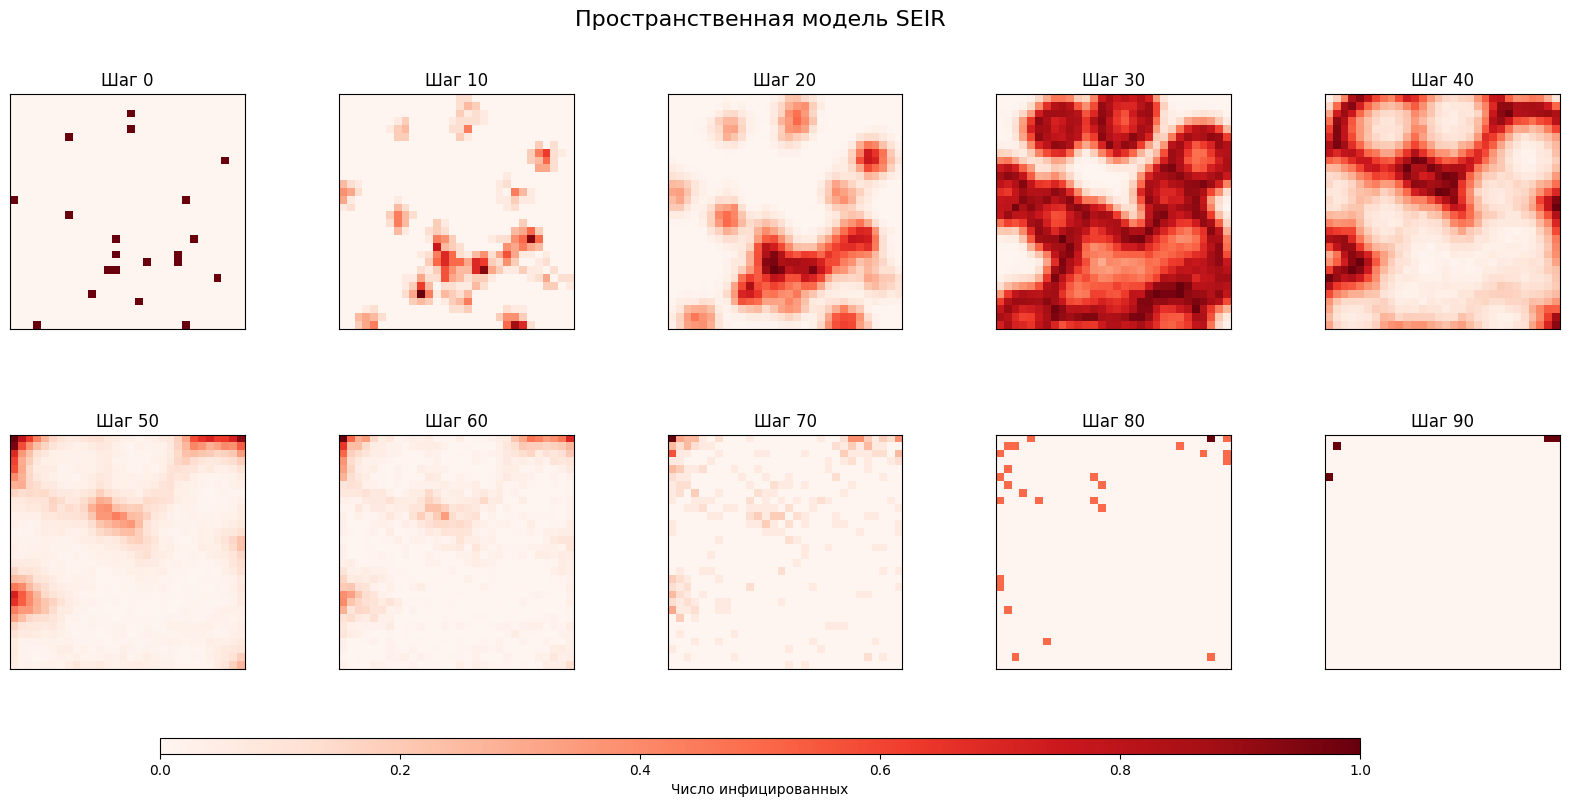
\includegraphics[scale=0.3]{images/graph03}
		\caption{Пространственные графики численной реализации вероятностной SEIR модели для гриппа}
		\label{fig:graph03}
	\end{figure}
	
\end{frame}

%--------------------------------------------------------------------------



\begin{frame}
	{Индивидуум-ориентированные и мультиагентные методы моделирования}
	\small{В модели, построенной на основе клеточных автоматов, используется решетка, где каждая ячейка представляет собой часть популяции. Однако в реальности индивиды имеют различные характеристики, например
	\begin{itemize}
		\item индивидуальная восприимчивость, то есть люди имеют разный иммунитет, что влияет на вероятность заражения;
		\item различные периоды инкубации и выздоровления, то есть у разных индивидов инкубационный и инфекционный периоды могут варьироваться;
		\item индивидуальные контакты, то есть люди взаимодействуют с разным числом других людей, что влияет на передачу болезни;
		\item мобильность, то есть люди перемещаются в пространстве (не фиксированы в одной ячейке).
	\end{itemize}
	
	Учет этих факторов может значительно повысить точность модели, так как она будет учитывать вариативность в поведении и характеристиках индивидов.}
\end{frame}

%--------------------------------------------------------------------------

\begin{frame}
	{Индивидуум-ориентированные и мультиагентные методы моделирования}
\begin{figure}
	\centering
	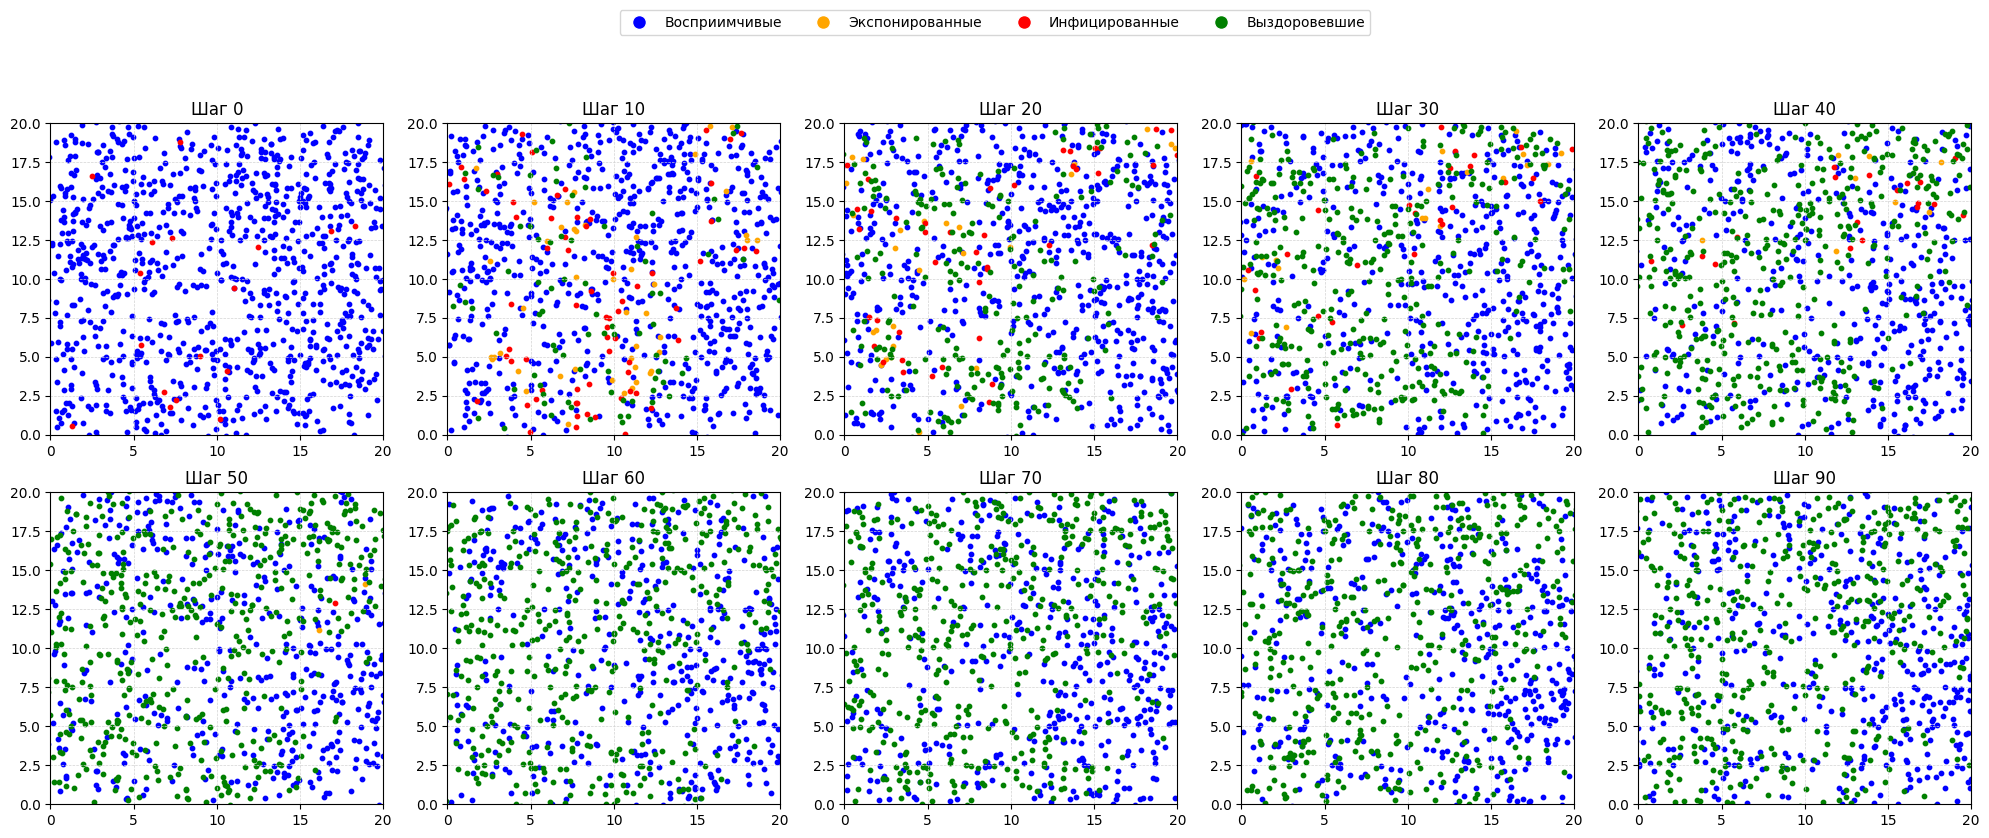
\includegraphics[scale=0.2]{images/graph04}
	\caption{Графическое представление реализации мультиагентной SEIR модели}
	\label{fig:graph04}
\end{figure}
\end{frame}

%--------------------------------------------------------------------------
\begin{frame}
	{Индивидуум-ориентированные и мультиагентные методы моделирования}
Таким образом, можно заметить, что теперь процесс распространения гриппа протекает иначе. Основной пик был между 10-ым и 20-ым днями, а далее после 60-го дня грипп не распространялся, то есть распространение прекратилось. Можно сделать выводы, что наличие у каждого индивида особых собственных свойств сильно сказывается на процессе распространения заболевания.
\end{frame}
%--------------------------------------------------------------------------

\begin{frame}
	{Заключение}
	В данной работе рассмотрена SEIR-модель и ее расширения, с помощью которых был смоделирован процесс распространения заболеваний.
	В ходе работы
	\begin{enumerate}
		\item рассмотрены расширения базовой SEIR модели: вероятностная модель, пространственная модель, мультиагентная модель;
		\item на практике были рассмотрены способы построения расширений для модели SEIR для решения задачи о моделировании распространения гриппа и приведены результаты моделирования.
	\end{enumerate}
\end{frame}

%--------------------------------------------------------------------------

\begin{frame}
	{Список используемых источников}
	\begin{enumerate}
		\item Statistical forecasting of the dynamics of epidemiological indicators for COVID-19 incidence in the Republic of Belarus / Yu. S. Kharin, V. A. Valoshka, O. V. Dernakova, V. I. Malugin, A. Yu. Kharin// Journal of the Belarusian State University. Mathematics and Informatics. - 2020. - № 3. - С. 36-50
		\item Methods of intellectual data analysis in COVID-19 research / O. V. Senko, A. V. Kuznetsova, E. M. Voronin, O. A. Kravtsova, L. R. Borisova, I. L. Kirilyuk, V. G. Akimkin// Journal of the Belarusian State University. Mathematics and Informatics. – 2022. – № 1. – С. 83-96
		\item Детерминированные и стохастические модели распространения инфекции и тестирование в изолированном контингенте/ Чигарев, А. В.,Журавков, М. А.,Чигарев, В. А.// Журнал Белорусского государственного университета. Математика. Информатика - 2021. - № 3. - С. 57-67
	\end{enumerate}
\end{frame}

%--------------------------------------------------------------------------

\end{document} 